\chapter{ผลการพัฒนา}
\label{chapter:result}

ทีม Manyfox มีการประเมินผลการพัฒนาโดยการวัดผลจาก 2 ด้านคือ เชิงประสิทธิภาพ และ เชิงประสิทธิผล
โดยมีวิธีการในการประเมินผลการพัฒนาดังนี้

\section{การประเมินผลเชิงประสิทธิภาพ}
การประเมินผลเชิงประสิทธิภาพใช้ เว็บไซต์ \textbf{https://web.dev} ที่เป็นเครื่องมือของ google ในการประเมินผลออกมาเป็นตัวเลข และแสดงถึงจุดบกพร่อง
โดยแยกออกมาเป็น 4 ด้านดังนี้
\begin{figure}[!htbp]
	\centering
	
\includegraphics[width=0.8\linewidth]{webdev-logo}
	\caption{Web.dev logo}
	(ที่มา:
	https://web.dev/
	)
	\label{Fig:wed-dev}
\end{figure}
\subsection{Performance}
ประเมินผลจากการตรวจสอบระยะเวลาการโหลดหน้าแรก (ส่วนที่มองเห็นครั้งแรกเมื่อเปิดหน้าเว็บไซต์)
\subsection{Accessibility}
ตรวจสอบปัญหาทั่วไปที่อาจมีผลถึงการะเข้าถึงเนื้อหาบทความ
\subsection{Best practices}
ตรวจสอบรูปแบบโค้ดทั้งหมด ที่ควรเขียนในแบบที่ควรเป็น
\subsection{SEO}
ตรวจสอบ Best practices เฉพาะในส่วน SEO เพื่อให้มั่นใจว่าสามารถค้นหาผ่านทาง Google search เจอ
\newpage
\begin{figure}[!htbp]
	\centering
	\subfigure[ผลการประเมิน Manyfox Web Appication]{
		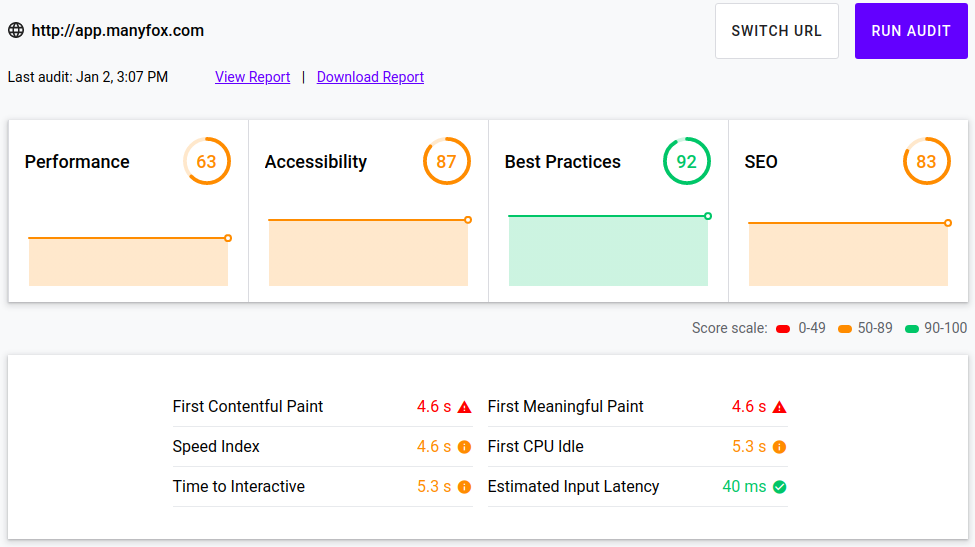
\includegraphics[width=1\linewidth]{audit-app}
		\label{Fig:audit-app}
	}
	\subfigure[ผลการะประเมิน Manyfox Web Landing page]{
		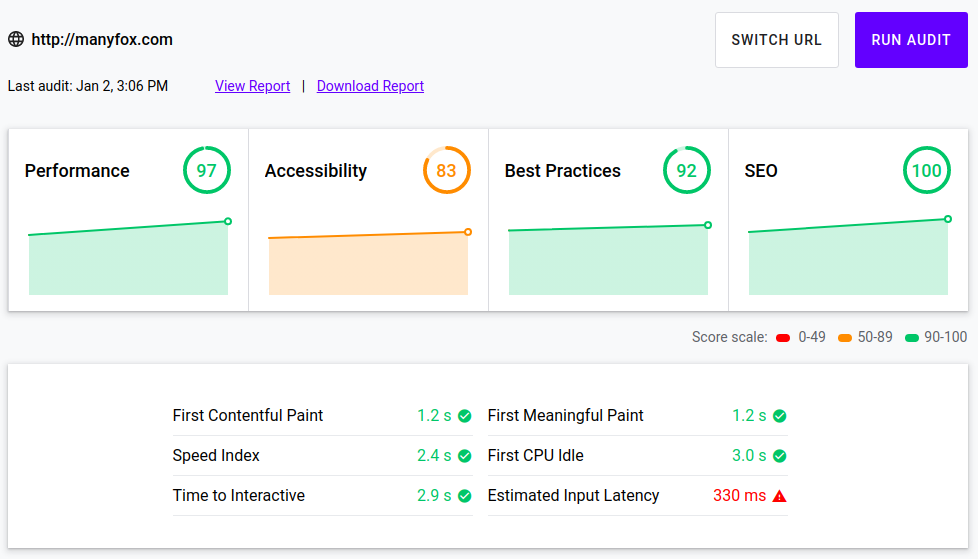
\includegraphics[width=1\linewidth]{audit-landing-page}
		\label{Fig:audit-landing-page}
	}
	\caption{ผลการประเมิน Manyfox}

\end{figure}

\section{การประเมินผลเชิงประสิทธิผล}
การประเมินผลเชิงประสิทธิผลโดยวัดจากความพึงพอใจของผู้ใช้ เพื่อให้เข้าถึงการรับฟังความเห็นจากผู้ใช้ได้มากขึ้น จึงพัฒนา Feedback page
เพื่อรับฟังความเห็น หรือปัญหาจากผู้ใช้ โดยมีวิธีการดังนี้
\subsection{เข้าที่หน้าเว็บไซต์ https://app.manyfox.com/feedback}
เขียนหัวข้อและเนื้อหา Feedback
\begin{figure}[!htbp]
	\centering
	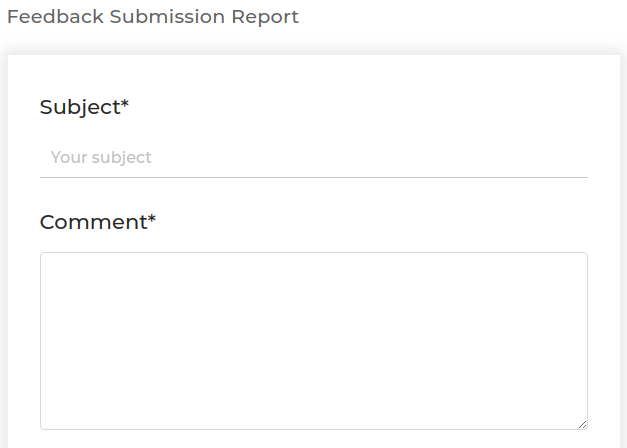
\includegraphics[width=0.8\linewidth]{feedback-1}
	\caption{ช่องสำหรับหัวข้อและเนื้อหา}
	\label{Fig:feedback-1}
\end{figure}
\subsection{อัพโหลดรูปภาพประกอบ}
หากมีรูปภาพประกอบสามารถอัพโหลดรูปภาพที่มีสกุลไฟล์ jpg png และ gif โดยมีขนาดไม่มากกว่า 2MB ต่อไฟล์ โดยสามารถอัพโหลดได้มากสุด 5 ไฟล์
\\
\begin{figure}[!htbp]
	\centering
	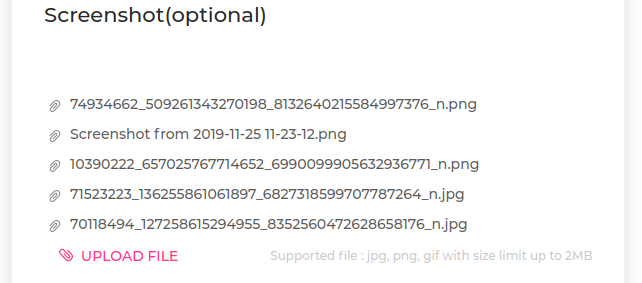
\includegraphics[width=0.8\linewidth]{feedback-2}
	\caption{ช่องอัพโหลดรูปภาพ}
	\label{Fig:wed-dev}
\end{figure}
\newpage
\subsection{Email ที่ต้องการติดต่อกลับ}
เมื่อทาง Manyfox แก้ไขหรือได้ตอบรับ Feedback จะติดต่อกลับผ่าน Email นี้ และกด Submit เป็นการเสร็จสิ้น
\begin{figure}[!htbp]
	\centering
	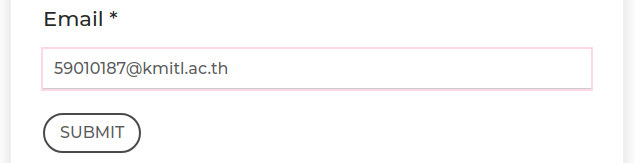
\includegraphics[width=0.8\linewidth]{feedback-3}
	\caption{ช่องกรอก Email}
	\label{Fig:wed-dev}
\end{figure}

\vskip1em
เมื่อทาง Manyfox ได้รับ Feedback จะมีข้อมูล Feedback ขึ้นใน Channel \#manyfox\-support\-email ใน workspace Nextzy
\begin{figure}[!htbp]
	\centering
	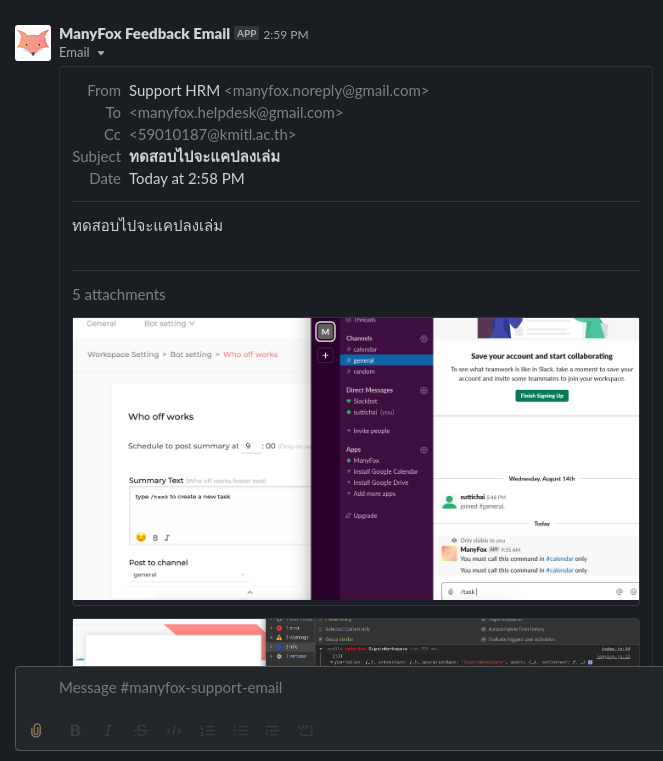
\includegraphics[width=0.8\linewidth]{feedback-4}
	\caption{Feedback ภายใน Slack}
	\label{Fig:wed-dev}
\end{figure}